\documentclass{standalone}
\usepackage{tikz}
\usetikzlibrary{patterns, positioning}
\usepackage[sfdefault]{ClearSans} %% option 'sfdefault' activates Clear Sans as the default text font
\usepackage[T1]{fontenc}

\begin{document}
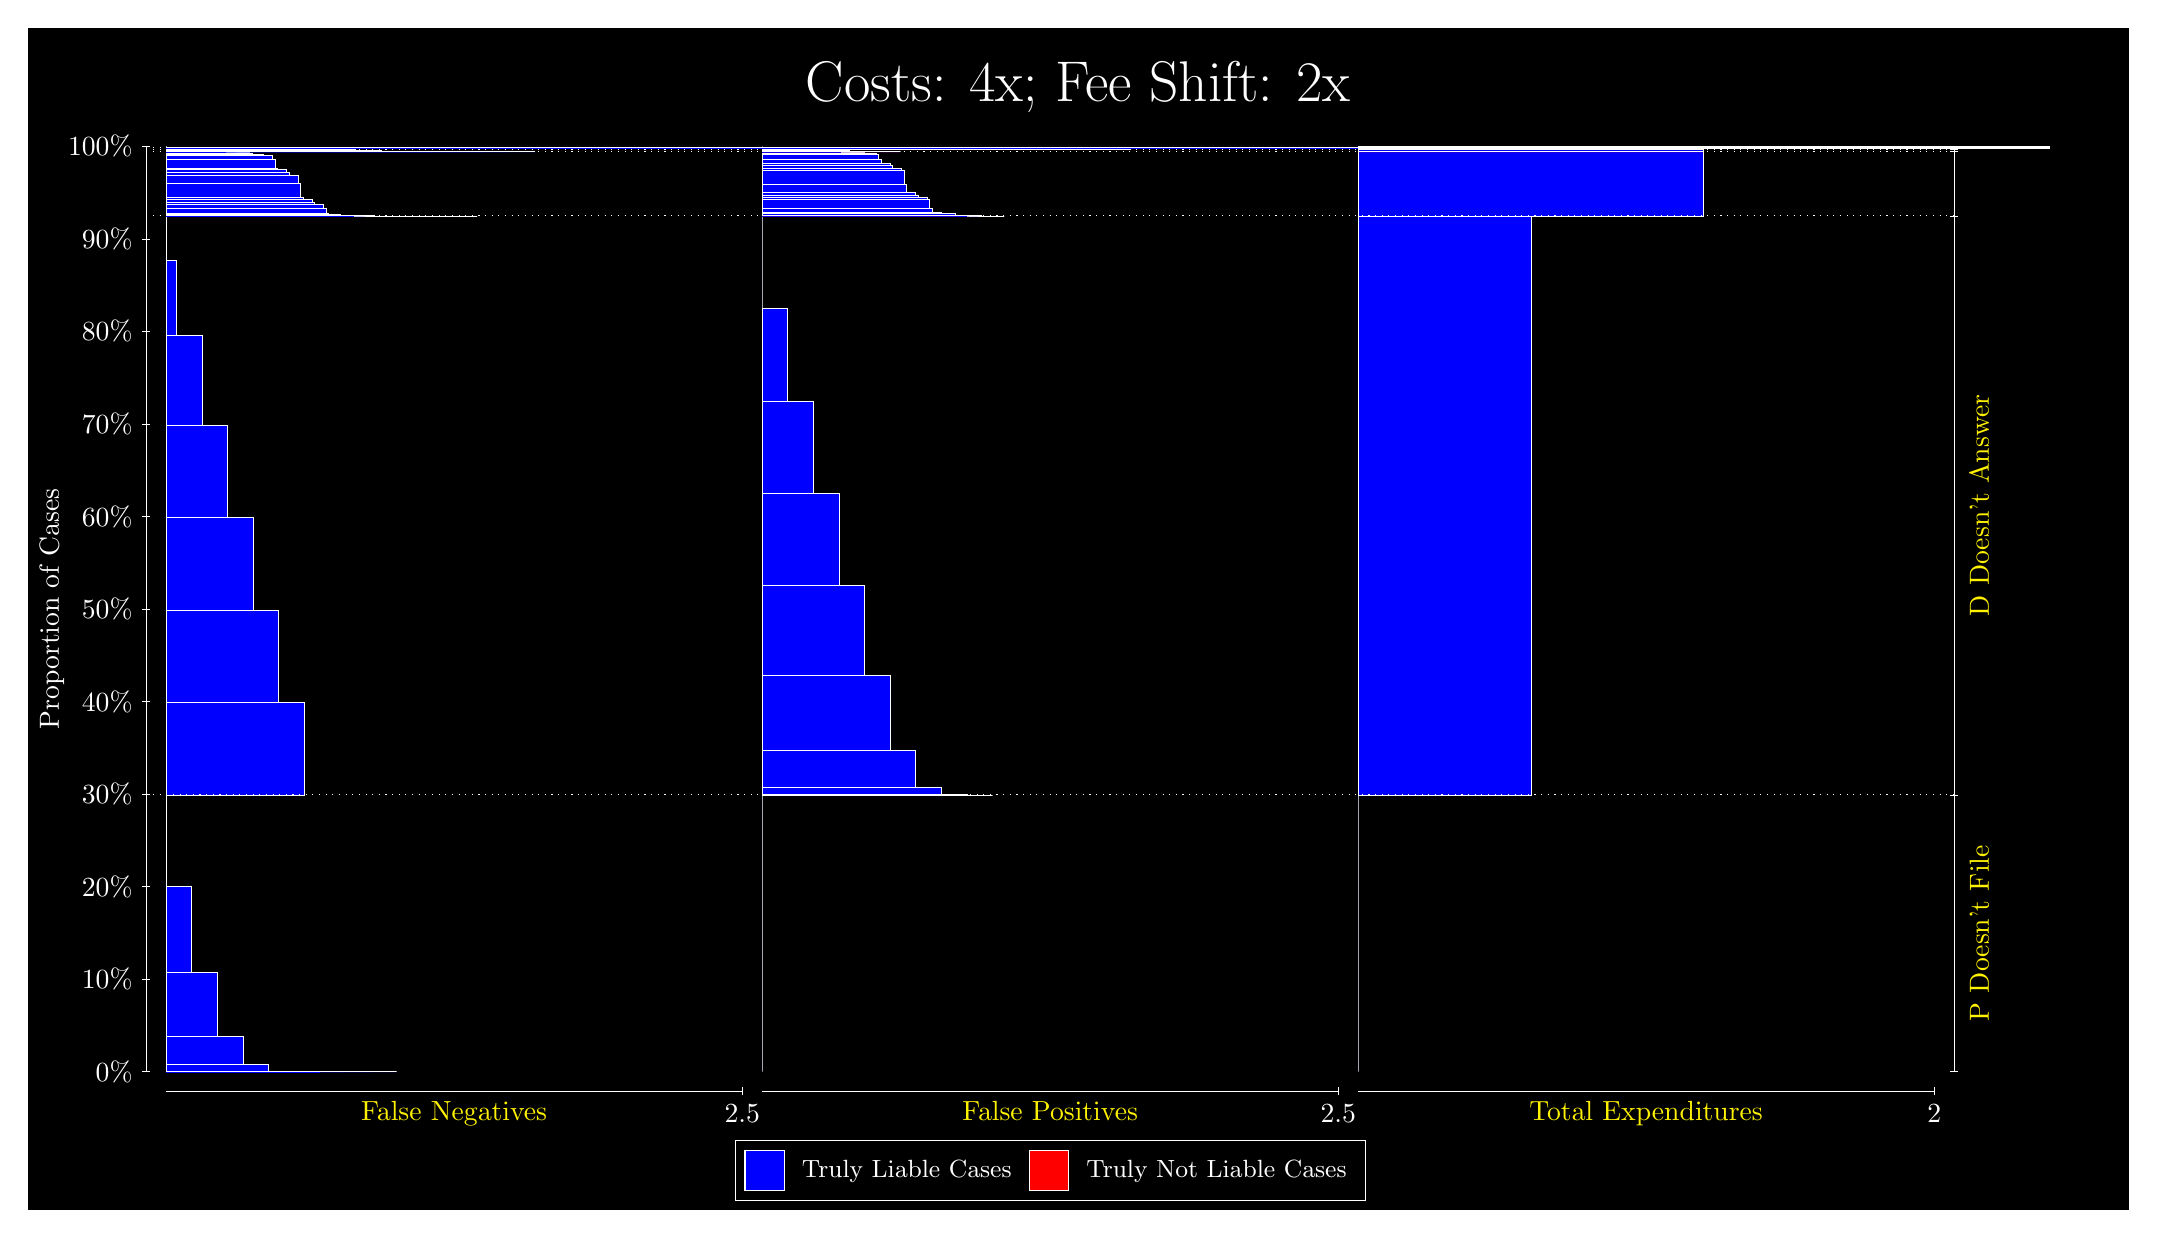
\begin{tikzpicture}
\draw[fill=black] (0,0) rectangle (26.667,15);
\draw[text=white] (0,13.5) rectangle (26.667,15) node[midway] {\huge Costs: 4x; Fee Shift: 2x};
\draw[white, very thin] (1.5,1.75) -- (1.5,13.5);
\node[rotate=90, text=white, anchor=center] at (0.3, 7.625) {Proportion of Cases};
\draw[white, very thin] (1.45,1.75) -- (1.55,1.75);
\node[text=white, anchor=east] at (1.45, 1.75) {0\%};
\draw[white, very thin] (1.45,2.925) -- (1.55,2.925);
\node[text=white, anchor=east] at (1.45, 2.925) {10\%};
\draw[white, very thin] (1.45,4.1) -- (1.55,4.1);
\node[text=white, anchor=east] at (1.45, 4.1) {20\%};
\draw[white, very thin] (1.45,5.275) -- (1.55,5.275);
\node[text=white, anchor=east] at (1.45, 5.275) {30\%};
\draw[white, very thin] (1.45,6.45) -- (1.55,6.45);
\node[text=white, anchor=east] at (1.45, 6.45) {40\%};
\draw[white, very thin] (1.45,7.625) -- (1.55,7.625);
\node[text=white, anchor=east] at (1.45, 7.625) {50\%};
\draw[white, very thin] (1.45,8.8) -- (1.55,8.8);
\node[text=white, anchor=east] at (1.45, 8.8) {60\%};
\draw[white, very thin] (1.45,9.975) -- (1.55,9.975);
\node[text=white, anchor=east] at (1.45, 9.975) {70\%};
\draw[white, very thin] (1.45,11.15) -- (1.55,11.15);
\node[text=white, anchor=east] at (1.45, 11.15) {80\%};
\draw[white, very thin] (1.45,12.325) -- (1.55,12.325);
\node[text=white, anchor=east] at (1.45, 12.325) {90\%};
\draw[white, very thin] (1.45,13.5) -- (1.55,13.5);
\node[text=white, anchor=east] at (1.45, 13.5) {100\%};

\draw[white, very thin] (24.457,1.75) -- (24.457,13.5);
\draw[white, very thin] (24.407,1.75) -- (24.507,1.75);
\node[anchor=west] at (24.407, 1.75) {};
\draw[white, very thin] (24.407,5.264) -- (24.507,5.264);
\node[anchor=west] at (24.407, 5.264) {};
\draw[white, very thin] (24.407,12.617) -- (24.507,12.617);
\node[anchor=west] at (24.407, 12.617) {};
\draw[white, very thin] (24.407,13.434) -- (24.507,13.434);
\node[anchor=west] at (24.407, 13.434) {};
\draw[white, very thin] (24.407,13.463) -- (24.507,13.463);
\node[anchor=west] at (24.407, 13.463) {};
\draw[white, very thin] (24.407,13.48) -- (24.507,13.48);
\node[anchor=west] at (24.407, 13.48) {};
\draw[white, very thin] (24.407,13.5) -- (24.507,13.5);
\node[anchor=west] at (24.407, 13.5) {};

\draw[white, very thin, fill=blue] (1.75,1.75) rectangle (4.6775,1.75);
\draw[white, very thin, fill=blue] (1.75,1.75) rectangle (4.3523,1.75);
\draw[white, very thin, fill=blue] (1.75,1.75) rectangle (4.027,1.75);
\draw[white, very thin, fill=blue] (1.75,1.75) rectangle (3.7017,1.7503);
\draw[white, very thin, fill=blue] (1.75,1.7503) rectangle (3.3764,1.7576);
\draw[white, very thin, fill=blue] (1.75,1.7576) rectangle (3.0511,1.8361);
\draw[white, very thin, fill=blue] (1.75,1.8361) rectangle (2.7258,2.1984);
\draw[white, very thin, fill=blue] (1.75,2.1984) rectangle (2.4006,3.0086);
\draw[white, very thin, fill=blue] (1.75,3.0086) rectangle (2.0753,4.0995);
\draw[white, very thin, fill=red] (1.75,4.0995) rectangle (1.75,4.0995);
\draw[white, very thin, fill=blue] (1.75,4.0995) rectangle (1.75,5.264);
\draw[white, very thin, fill=blue] (1.75,5.264) rectangle (3.5065,6.439);
\draw[white, very thin, fill=blue] (1.75,6.439) rectangle (3.1812,7.614);
\draw[white, very thin, fill=blue] (1.75,7.614) rectangle (2.856,8.7889);
\draw[white, very thin, fill=blue] (1.75,8.7889) rectangle (2.5307,9.9614);
\draw[white, very thin, fill=blue] (1.75,9.9614) rectangle (2.2054,11.102);
\draw[white, very thin, fill=blue] (1.75,11.102) rectangle (1.8801,12.05);
\draw[white, very thin, fill=red] (1.75,12.05) rectangle (1.75,12.05);
\draw[white, very thin, fill=blue] (1.75,12.05) rectangle (1.75,12.617);
\draw[white, very thin, fill=blue] (1.75,12.617) rectangle (5.7022,12.617);
\draw[white, very thin, fill=blue] (1.75,12.617) rectangle (5.5558,12.617);
\draw[white, very thin, fill=blue] (1.75,12.617) rectangle (5.4094,12.617);
\draw[white, very thin, fill=blue] (1.75,12.617) rectangle (5.3769,12.617);
\draw[white, very thin, fill=blue] (1.75,12.617) rectangle (5.2631,12.617);
\draw[white, very thin, fill=blue] (1.75,12.617) rectangle (5.2305,12.617);
\draw[white, very thin, fill=blue] (1.75,12.617) rectangle (5.1167,12.617);
\draw[white, very thin, fill=blue] (1.75,12.617) rectangle (5.0842,12.617);
\draw[white, very thin, fill=blue] (1.75,12.617) rectangle (5.0516,12.617);
\draw[white, very thin, fill=blue] (1.75,12.617) rectangle (4.9378,12.617);
\draw[white, very thin, fill=blue] (1.75,12.617) rectangle (4.9052,12.617);
\draw[white, very thin, fill=blue] (1.75,12.617) rectangle (4.7914,12.617);
\draw[white, very thin, fill=blue] (1.75,12.617) rectangle (4.7589,12.617);
\draw[white, very thin, fill=blue] (1.75,12.617) rectangle (4.7263,12.617);
\draw[white, very thin, fill=blue] (1.75,12.617) rectangle (4.6125,12.617);
\draw[white, very thin, fill=blue] (1.75,12.617) rectangle (4.58,12.617);
\draw[white, very thin, fill=blue] (1.75,12.617) rectangle (4.4661,12.617);
\draw[white, very thin, fill=blue] (1.75,12.617) rectangle (4.4336,12.617);
\draw[white, very thin, fill=blue] (1.75,12.617) rectangle (4.4011,12.618);
\draw[white, very thin, fill=blue] (1.75,12.618) rectangle (4.2872,12.618);
\draw[white, very thin, fill=blue] (1.75,12.618) rectangle (4.2547,12.618);
\draw[white, very thin, fill=blue] (1.75,12.618) rectangle (4.1408,12.619);
\draw[white, very thin, fill=blue] (1.75,12.619) rectangle (4.1083,12.624);
\draw[white, very thin, fill=blue] (1.75,12.624) rectangle (4.0758,12.63);
\draw[white, very thin, fill=blue] (1.75,12.63) rectangle (3.9619,12.635);
\draw[white, very thin, fill=blue] (1.75,12.635) rectangle (3.9294,12.643);
\draw[white, very thin, fill=blue] (1.75,12.643) rectangle (3.8155,12.653);
\draw[white, very thin, fill=blue] (1.75,12.653) rectangle (3.783,12.713);
\draw[white, very thin, fill=blue] (1.75,12.713) rectangle (3.7505,12.766);
\draw[white, very thin, fill=blue] (1.75,12.766) rectangle (3.6366,12.795);
\draw[white, very thin, fill=blue] (1.75,12.795) rectangle (3.6041,12.83);
\draw[white, very thin, fill=blue] (1.75,12.83) rectangle (3.4903,12.859);
\draw[white, very thin, fill=blue] (1.75,12.859) rectangle (3.4577,13.028);
\draw[white, very thin, fill=blue] (1.75,13.028) rectangle (3.4252,13.138);
\draw[white, very thin, fill=blue] (1.75,13.138) rectangle (3.3114,13.174);
\draw[white, very thin, fill=blue] (1.75,13.174) rectangle (3.2788,13.204);
\draw[white, very thin, fill=blue] (1.75,13.204) rectangle (3.165,13.225);
\draw[white, very thin, fill=blue] (1.75,13.225) rectangle (3.1325,13.333);
\draw[white, very thin, fill=blue] (1.75,13.333) rectangle (3.0999,13.389);
\draw[white, very thin, fill=blue] (1.75,13.389) rectangle (2.9861,13.399);
\draw[white, very thin, fill=blue] (1.75,13.399) rectangle (2.9535,13.404);
\draw[white, very thin, fill=blue] (1.75,13.404) rectangle (2.8397,13.408);
\draw[white, very thin, fill=blue] (1.75,13.408) rectangle (2.8072,13.423);
\draw[white, very thin, fill=blue] (1.75,13.423) rectangle (2.7746,13.433);
\draw[white, very thin, fill=blue] (1.75,13.433) rectangle (2.6608,13.433);
\draw[white, very thin, fill=blue] (1.75,13.433) rectangle (2.6283,13.433);
\draw[white, very thin, fill=blue] (1.75,13.433) rectangle (2.5144,13.434);
\draw[white, very thin, fill=blue] (1.75,13.434) rectangle (2.4819,13.434);
\draw[white, very thin, fill=blue] (1.75,13.434) rectangle (2.3355,13.434);
\draw[white, very thin, fill=blue] (1.75,13.434) rectangle (2.1891,13.434);
\draw[white, very thin, fill=red] (1.75,13.434) rectangle (1.75,13.434);
\draw[white, very thin, fill=blue] (1.75,13.434) rectangle (6.4341,13.434);
\draw[white, very thin, fill=blue] (1.75,13.434) rectangle (6.1088,13.434);
\draw[white, very thin, fill=blue] (1.75,13.434) rectangle (5.7835,13.434);
\draw[white, very thin, fill=blue] (1.75,13.434) rectangle (5.4582,13.434);
\draw[white, very thin, fill=blue] (1.75,13.434) rectangle (5.1329,13.434);
\draw[white, very thin, fill=blue] (1.75,13.434) rectangle (4.8077,13.437);
\draw[white, very thin, fill=blue] (1.75,13.437) rectangle (4.4824,13.449);
\draw[white, very thin, fill=blue] (1.75,13.449) rectangle (4.1571,13.461);
\draw[white, very thin, fill=blue] (1.75,13.461) rectangle (3.8318,13.463);
\draw[white, very thin, fill=blue] (1.75,13.463) rectangle (3.5065,13.463);
\draw[white, very thin, fill=red] (1.75,13.463) rectangle (1.75,13.463);
\draw[white, very thin, fill=blue] (1.75,13.463) rectangle (3.5065,13.463);
\draw[white, very thin, fill=blue] (1.75,13.463) rectangle (3.1812,13.463);
\draw[white, very thin, fill=blue] (1.75,13.463) rectangle (2.856,13.463);
\draw[white, very thin, fill=blue] (1.75,13.463) rectangle (2.5307,13.464);
\draw[white, very thin, fill=blue] (1.75,13.464) rectangle (2.2054,13.469);
\draw[white, very thin, fill=blue] (1.75,13.469) rectangle (1.8801,13.475);
\draw[white, very thin, fill=red] (1.75,13.475) rectangle (1.75,13.475);
\draw[white, very thin, fill=blue] (1.75,13.475) rectangle (1.75,13.48);
\draw[white, very thin, fill=blue] (1.75,13.48) rectangle (15.217,13.48);
\draw[white, very thin, fill=blue] (1.75,13.48) rectangle (14.891,13.48);
\draw[white, very thin, fill=blue] (1.75,13.48) rectangle (14.566,13.48);
\draw[white, very thin, fill=blue] (1.75,13.48) rectangle (14.241,13.48);
\draw[white, very thin, fill=blue] (1.75,13.48) rectangle (14.241,13.48);
\draw[white, very thin, fill=blue] (1.75,13.48) rectangle (13.916,13.48);
\draw[white, very thin, fill=blue] (1.75,13.48) rectangle (13.59,13.48);
\draw[white, very thin, fill=blue] (1.75,13.48) rectangle (13.265,13.48);
\draw[white, very thin, fill=blue] (1.75,13.48) rectangle (13.265,13.481);
\draw[white, very thin, fill=blue] (1.75,13.481) rectangle (12.94,13.483);
\draw[white, very thin, fill=blue] (1.75,13.483) rectangle (12.94,13.483);
\draw[white, very thin, fill=blue] (1.75,13.483) rectangle (12.614,13.485);
\draw[white, very thin, fill=blue] (1.75,13.485) rectangle (12.614,13.486);
\draw[white, very thin, fill=blue] (1.75,13.486) rectangle (12.289,13.488);
\draw[white, very thin, fill=blue] (1.75,13.488) rectangle (11.964,13.489);
\draw[white, very thin, fill=blue] (1.75,13.489) rectangle (11.639,13.489);
\draw[white, very thin, fill=blue] (1.75,13.489) rectangle (11.313,13.489);
\draw[white, very thin, fill=blue] (1.75,13.489) rectangle (10.988,13.489);
\draw[white, very thin, fill=red] (1.75,13.489) rectangle (1.75,13.489);
\draw[white, very thin, fill=blue] (1.75,13.489) rectangle (1.75,13.5);
\draw[white, very thin, fill=red] (9.3189,1.75) rectangle (9.3189,1.75);
\draw[white, very thin, fill=blue] (9.3189,1.75) rectangle (9.3189,5.264);
\draw[white, very thin, fill=red] (9.3189,5.264) rectangle (12.246,5.264);
\draw[white, very thin, fill=blue] (9.3189,5.264) rectangle (12.246,5.264);
\draw[white, very thin, fill=blue] (9.3189,5.264) rectangle (11.921,5.2685);
\draw[white, very thin, fill=blue] (9.3189,5.2685) rectangle (11.596,5.3567);
\draw[white, very thin, fill=blue] (9.3189,5.3567) rectangle (11.271,5.8309);
\draw[white, very thin, fill=blue] (9.3189,5.8309) rectangle (10.945,6.7794);
\draw[white, very thin, fill=blue] (9.3189,6.7794) rectangle (10.62,7.9198);
\draw[white, very thin, fill=blue] (9.3189,7.9198) rectangle (10.295,9.0923);
\draw[white, very thin, fill=blue] (9.3189,9.0923) rectangle (9.9694,10.267);
\draw[white, very thin, fill=blue] (9.3189,10.267) rectangle (9.6442,11.442);
\draw[white, very thin, fill=blue] (9.3189,11.442) rectangle (9.3189,12.617);
\draw[white, very thin, fill=red] (9.3189,12.617) rectangle (12.393,12.617);
\draw[white, very thin, fill=blue] (9.3189,12.617) rectangle (12.393,12.617);
\draw[white, very thin, fill=red] (9.3189,12.617) rectangle (12.246,12.617);
\draw[white, very thin, fill=blue] (9.3189,12.617) rectangle (12.246,12.617);
\draw[white, very thin, fill=red] (9.3189,12.617) rectangle (12.1,12.617);
\draw[white, very thin, fill=blue] (9.3189,12.617) rectangle (12.1,12.618);
\draw[white, very thin, fill=blue] (9.3189,12.618) rectangle (12.068,12.618);
\draw[white, very thin, fill=red] (9.3189,12.618) rectangle (11.954,12.618);
\draw[white, very thin, fill=blue] (9.3189,12.618) rectangle (11.954,12.618);
\draw[white, very thin, fill=blue] (9.3189,12.618) rectangle (11.921,12.619);
\draw[white, very thin, fill=red] (9.3189,12.619) rectangle (11.807,12.619);
\draw[white, very thin, fill=blue] (9.3189,12.619) rectangle (11.807,12.628);
\draw[white, very thin, fill=blue] (9.3189,12.628) rectangle (11.775,12.644);
\draw[white, very thin, fill=blue] (9.3189,12.644) rectangle (11.742,12.648);
\draw[white, very thin, fill=blue] (9.3189,12.648) rectangle (11.628,12.653);
\draw[white, very thin, fill=blue] (9.3189,12.653) rectangle (11.596,12.663);
\draw[white, very thin, fill=blue] (9.3189,12.663) rectangle (11.482,12.718);
\draw[white, very thin, fill=blue] (9.3189,12.718) rectangle (11.449,12.826);
\draw[white, very thin, fill=blue] (9.3189,12.826) rectangle (11.417,12.848);
\draw[white, very thin, fill=blue] (9.3189,12.848) rectangle (11.303,12.877);
\draw[white, very thin, fill=blue] (9.3189,12.877) rectangle (11.271,12.914);
\draw[white, very thin, fill=blue] (9.3189,12.914) rectangle (11.157,13.023);
\draw[white, very thin, fill=blue] (9.3189,13.023) rectangle (11.124,13.192);
\draw[white, very thin, fill=blue] (9.3189,13.192) rectangle (11.092,13.222);
\draw[white, very thin, fill=blue] (9.3189,13.222) rectangle (10.978,13.256);
\draw[white, very thin, fill=blue] (9.3189,13.256) rectangle (10.945,13.285);
\draw[white, very thin, fill=blue] (9.3189,13.285) rectangle (10.831,13.338);
\draw[white, very thin, fill=blue] (9.3189,13.338) rectangle (10.799,13.398);
\draw[white, very thin, fill=blue] (9.3189,13.398) rectangle (10.766,13.409);
\draw[white, very thin, fill=blue] (9.3189,13.409) rectangle (10.653,13.416);
\draw[white, very thin, fill=blue] (9.3189,13.416) rectangle (10.62,13.422);
\draw[white, very thin, fill=blue] (9.3189,13.422) rectangle (10.506,13.428);
\draw[white, very thin, fill=blue] (9.3189,13.428) rectangle (10.474,13.433);
\draw[white, very thin, fill=blue] (9.3189,13.433) rectangle (10.441,13.433);
\draw[white, very thin, fill=blue] (9.3189,13.433) rectangle (10.327,13.434);
\draw[white, very thin, fill=blue] (9.3189,13.434) rectangle (10.295,13.434);
\draw[white, very thin, fill=blue] (9.3189,13.434) rectangle (10.181,13.434);
\draw[white, very thin, fill=blue] (9.3189,13.434) rectangle (10.148,13.434);
\draw[white, very thin, fill=blue] (9.3189,13.434) rectangle (10.116,13.434);
\draw[white, very thin, fill=blue] (9.3189,13.434) rectangle (10.002,13.434);
\draw[white, very thin, fill=blue] (9.3189,13.434) rectangle (9.9694,13.434);
\draw[white, very thin, fill=blue] (9.3189,13.434) rectangle (9.8556,13.434);
\draw[white, very thin, fill=blue] (9.3189,13.434) rectangle (9.8231,13.434);
\draw[white, very thin, fill=blue] (9.3189,13.434) rectangle (9.7905,13.434);
\draw[white, very thin, fill=blue] (9.3189,13.434) rectangle (9.6767,13.434);
\draw[white, very thin, fill=blue] (9.3189,13.434) rectangle (9.6442,13.434);
\draw[white, very thin, fill=blue] (9.3189,13.434) rectangle (9.5303,13.434);
\draw[white, very thin, fill=blue] (9.3189,13.434) rectangle (9.4978,13.434);
\draw[white, very thin, fill=blue] (9.3189,13.434) rectangle (9.4652,13.434);
\draw[white, very thin, fill=blue] (9.3189,13.434) rectangle (9.3514,13.434);
\draw[white, very thin, fill=blue] (9.3189,13.434) rectangle (9.3189,13.434);
\draw[white, very thin, fill=red] (9.3189,13.434) rectangle (11.075,13.434);
\draw[white, very thin, fill=blue] (9.3189,13.434) rectangle (11.075,13.434);
\draw[white, very thin, fill=blue] (9.3189,13.434) rectangle (10.75,13.437);
\draw[white, very thin, fill=blue] (9.3189,13.437) rectangle (10.425,13.449);
\draw[white, very thin, fill=blue] (9.3189,13.449) rectangle (10.1,13.461);
\draw[white, very thin, fill=blue] (9.3189,13.461) rectangle (9.7743,13.463);
\draw[white, very thin, fill=blue] (9.3189,13.463) rectangle (9.449,13.463);
\draw[white, very thin, fill=blue] (9.3189,13.463) rectangle (9.3189,13.463);
\draw[white, very thin, fill=red] (9.3189,13.463) rectangle (14.003,13.463);
\draw[white, very thin, fill=blue] (9.3189,13.463) rectangle (14.003,13.463);
\draw[white, very thin, fill=blue] (9.3189,13.463) rectangle (13.678,13.463);
\draw[white, very thin, fill=blue] (9.3189,13.463) rectangle (13.352,13.464);
\draw[white, very thin, fill=blue] (9.3189,13.464) rectangle (13.027,13.469);
\draw[white, very thin, fill=blue] (9.3189,13.469) rectangle (12.702,13.475);
\draw[white, very thin, fill=blue] (9.3189,13.475) rectangle (12.377,13.479);
\draw[white, very thin, fill=blue] (9.3189,13.479) rectangle (12.051,13.48);
\draw[white, very thin, fill=blue] (9.3189,13.48) rectangle (11.726,13.48);
\draw[white, very thin, fill=blue] (9.3189,13.48) rectangle (11.401,13.48);
\draw[white, very thin, fill=blue] (9.3189,13.48) rectangle (11.075,13.48);
\draw[white, very thin, fill=red] (9.3189,13.48) rectangle (22.786,13.48);
\draw[white, very thin, fill=blue] (9.3189,13.48) rectangle (22.786,13.48);
\draw[white, very thin, fill=red] (9.3189,13.48) rectangle (22.46,13.48);
\draw[white, very thin, fill=blue] (9.3189,13.48) rectangle (22.46,13.48);
\draw[white, very thin, fill=blue] (9.3189,13.48) rectangle (22.135,13.48);
\draw[white, very thin, fill=red] (9.3189,13.48) rectangle (22.135,13.48);
\draw[white, very thin, fill=blue] (9.3189,13.48) rectangle (22.135,13.48);
\draw[white, very thin, fill=red] (9.3189,13.48) rectangle (21.81,13.48);
\draw[white, very thin, fill=blue] (9.3189,13.48) rectangle (21.81,13.48);
\draw[white, very thin, fill=blue] (9.3189,13.48) rectangle (21.484,13.48);
\draw[white, very thin, fill=red] (9.3189,13.48) rectangle (21.484,13.48);
\draw[white, very thin, fill=blue] (9.3189,13.48) rectangle (21.484,13.48);
\draw[white, very thin, fill=red] (9.3189,13.48) rectangle (21.159,13.48);
\draw[white, very thin, fill=blue] (9.3189,13.48) rectangle (21.159,13.48);
\draw[white, very thin, fill=blue] (9.3189,13.48) rectangle (20.834,13.48);
\draw[white, very thin, fill=red] (9.3189,13.48) rectangle (20.834,13.48);
\draw[white, very thin, fill=blue] (9.3189,13.48) rectangle (20.834,13.481);
\draw[white, very thin, fill=blue] (9.3189,13.481) rectangle (20.834,13.481);
\draw[white, very thin, fill=blue] (9.3189,13.481) rectangle (20.509,13.481);
\draw[white, very thin, fill=blue] (9.3189,13.481) rectangle (20.509,13.482);
\draw[white, very thin, fill=blue] (9.3189,13.482) rectangle (20.509,13.483);
\draw[white, very thin, fill=blue] (9.3189,13.483) rectangle (20.183,13.484);
\draw[white, very thin, fill=blue] (9.3189,13.484) rectangle (20.183,13.486);
\draw[white, very thin, fill=blue] (9.3189,13.486) rectangle (20.183,13.487);
\draw[white, very thin, fill=blue] (9.3189,13.487) rectangle (19.858,13.487);
\draw[white, very thin, fill=blue] (9.3189,13.487) rectangle (19.858,13.49);
\draw[white, very thin, fill=blue] (9.3189,13.49) rectangle (19.533,13.491);
\draw[white, very thin, fill=blue] (9.3189,13.491) rectangle (19.533,13.491);
\draw[white, very thin, fill=blue] (9.3189,13.491) rectangle (19.207,13.491);
\draw[white, very thin, fill=blue] (9.3189,13.491) rectangle (19.207,13.491);
\draw[white, very thin, fill=blue] (9.3189,13.491) rectangle (18.882,13.491);
\draw[white, very thin, fill=blue] (9.3189,13.491) rectangle (18.882,13.491);
\draw[white, very thin, fill=blue] (9.3189,13.491) rectangle (18.557,13.491);
\draw[white, very thin, fill=blue] (9.3189,13.491) rectangle (18.557,13.491);
\draw[white, very thin, fill=blue] (9.3189,13.491) rectangle (18.232,13.491);
\draw[white, very thin, fill=blue] (9.3189,13.491) rectangle (17.906,13.491);
\draw[white, very thin, fill=red] (9.3189,13.491) rectangle (9.3189,13.491);
\draw[white, very thin, fill=blue] (9.3189,13.491) rectangle (9.3189,13.5);
\draw[white, very thin, fill=red] (16.888,1.75) rectangle (16.888,1.75);
\draw[white, very thin, fill=blue] (16.888,1.75) rectangle (16.888,5.264);
\draw[white, very thin, fill=red] (16.888,5.264) rectangle (19.083,5.264);
\draw[white, very thin, fill=blue] (16.888,5.264) rectangle (19.083,12.617);
\draw[white, very thin, fill=red] (16.888,12.617) rectangle (21.279,12.617);
\draw[white, very thin, fill=blue] (16.888,12.617) rectangle (21.279,13.434);
\draw[white, very thin, fill=red] (16.888,13.434) rectangle (21.279,13.434);
\draw[white, very thin, fill=blue] (16.888,13.434) rectangle (21.279,13.463);
\draw[white, very thin, fill=red] (16.888,13.463) rectangle (21.279,13.463);
\draw[white, very thin, fill=blue] (16.888,13.463) rectangle (21.279,13.48);
\draw[white, very thin, fill=red] (16.888,13.48) rectangle (25.67,13.48);
\draw[white, very thin, fill=blue] (16.888,13.48) rectangle (25.67,13.48);
\draw[white, very thin, fill=red] (16.888,13.48) rectangle (25.67,13.48);
\draw[white, very thin, fill=blue] (16.888,13.48) rectangle (25.67,13.488);
\draw[white, very thin, fill=red] (16.888,13.488) rectangle (25.67,13.488);
\draw[white, very thin, fill=blue] (16.888,13.488) rectangle (25.67,13.5);
\draw[white, dotted] (1.5,5.264) -- (24.457,5.264);
\draw[white, dotted] (1.5,12.617) -- (24.457,12.617);
\draw[white, dotted] (1.5,13.434) -- (24.457,13.434);
\draw[white, dotted] (1.5,13.463) -- (24.457,13.463);
\draw[white, dotted] (1.5,13.48) -- (24.457,13.48);
\draw[white, very thin] (1.75,1.5) -- (9.0689,1.5);
\node[text=yellow, anchor=north] at (5.4094, 1.5) {False Negatives};
\draw[white, very thin] (9.0689,1.45) -- (9.0689,1.55);
\node[text=white, anchor=north] at (9.0689, 1.45) {2.5};

\draw[white, very thin] (9.3189,1.5) -- (16.638,1.5);
\node[text=yellow, anchor=north] at (12.978, 1.5) {False Positives};
\draw[white, very thin] (16.638,1.45) -- (16.638,1.55);
\node[text=white, anchor=north] at (16.638, 1.45) {2.5};

\draw[white, very thin] (16.888,1.5) -- (24.207,1.5);
\node[text=yellow, anchor=north] at (20.547, 1.5) {Total Expenditures};
\draw[white, very thin] (24.207,1.45) -- (24.207,1.55);
\node[text=white, anchor=north] at (24.207, 1.45) {2};

\node[text=yellow, centered, rotate=90] at (24.777, 3.507) {P Doesn't File};
\node[text=yellow, centered, rotate=90] at (24.777, 8.9406) {D Doesn't Answer};





\draw (12.978300999999998,1.5) node[draw=none] (baseCoordinate) {};
\begin{scope}[align=center]
        \matrix[scale=0.5, draw=white, below=0.5cm of baseCoordinate, nodes={draw}, column sep=0.1cm]{
            \node[rectangle, draw, minimum width=0.5cm, minimum height=0.5cm, fill=blue] {}; &
            \node[draw=none, font=\small, text=white] (B) {Truly Liable Cases}; &
            \node[rectangle, draw, minimum width=0.5cm, minimum height=0.5cm, fill=red] {}; &
            \node[draw=none, font=\small, text=white] (B) {Truly Not Liable Cases}; \\
            };
\end{scope}

\end{tikzpicture}
\end{document}